% Research Note 02 -- Calendar-aware forecasting: EWMA baseline + explicit holiday model
% Compile: pdflatex note02_calendar_aware.tex  (run twice for refs)
% Figures in ./figures/ produced by src/eda_holiday.py (fig6, fig7).
\documentclass[11pt]{article}
\usepackage[margin=1in]{geometry}
\usepackage{amsmath,amssymb}
\usepackage{graphicx}
\usepackage{booktabs}
\usepackage{float}
\usepackage{xcolor}
\usepackage[colorlinks=true,linkcolor=blue,urlcolor=blue]{hyperref}
\graphicspath{{figures/}}

\newcommand{\veh}{\,\text{veh/h}}
\title{\textbf{Research Note 02}\\[2pt]
Calendar-Aware Forecasting:\\ EWMA Baseline and an Explicit Holiday Model}
\author{Traffic Forecasting Project}
\date{June 14, 2026}

\begin{document}
\maketitle

\begin{abstract}
\noindent
Building on Note 01 (the 4-week seasonal baseline explains $\sim$94\% of hourly
flow variance), we push past the $R^2\approx0.94$ wall with two interpretable,
leakage-safe refinements. (1) An \textbf{EWMA weekly baseline} replaces the flat
4-week mean with a single learned decay, capturing the ``recent weeks matter
more'' effect. (2) An \textbf{explicit holiday model} -- a pooled
per-(holiday, hour-of-day) multiplicative factor on the baseline -- targets the
fact that holidays are $8\%$ of hours but $\sim$23\% of squared error. In a
rolling-origin backtest on 2019, the combined model reaches
$\mathbf{R^2=0.9493}$ (vs.\ $0.9404$ flat), cutting holiday-window RMSE from
$67$ to $48\veh$ while leaving ordinary hours untouched. Per-sensor holiday
factors reveal real corridor heterogeneity (recreational routes \emph{gain}
traffic) but add little with only two training years. We then bound the headroom
of every endogenous lever -- autoregressive (ARIMA-style) residual modeling and
learned calendar/sensor features (ridge/XGBoost) -- and find all of it small
($\le+0.003\,R^2$). An oracle floor analysis shows our out-of-sample model
already matches the best \emph{in-sample} seasonal$+$holiday fit, so the residual
is dominated by irreducible noise: the one-week-ahead problem is, for this slice,
\textbf{effectively solved} ($R^2=0.949$, weekly-aggregate MAPE $3.55\%$). The
open questions are scope -- a small weather lever, and generalization (2020,
post-2022, other regions, speed).
\end{abstract}

\section*{Key findings}
\begin{itemize}
\item \textbf{EWMA baseline} (one decay parameter $\alpha\approx0.8$): $R^2$
  $0.9404\!\to\!0.9435$. Free weekly weights do no better -- one knob suffices.
\item A YoY-growth-adjusted ``last-year'' term is \textbf{secretly a holiday
  model}: its benefit concentrates almost entirely on holiday windows.
\item \textbf{Explicit holiday model}: holiday-window RMSE $67\!\to\!48\veh$
  ($-29\%$), \emph{surgical} (ordinary hours unchanged), and \textbf{stacks}
  with EWMA $\Rightarrow R^2=0.9493$.
\item Holiday response is \textbf{heterogeneous} across corridors, but with two
  training years the per-sensor refinement is marginal ($+0.0003\,R^2$) -- a
  ``needs more data'' win.
\item \textbf{Autoregressive headroom is small.} Recent-lag predictability is
  strong at $h{=}1$ ($R^2{=}0.63$) but collapses by a week out (aggregate ceiling
  $+0.0027$); weekly aggregation is cleaner (ACF $0.30$) but caps at $+0.0010$.
\item \textbf{ML on residual features does not help:} sub-daily calendar features
  are zero by construction; week-of-year is tiny and redundant; high-cardinality
  features overfit. The escalation to XGBoost is unwarranted.
\item \textbf{We are at the practical ceiling.} The out-of-sample model
  ($R^2{=}0.949$) already exceeds the best \emph{in-sample} static seasonal$+$
  holiday oracle; the residual is dominated by irreducible noise. Weekly-aggregate
  MAPE is $3.55\%$ (hourly MAPE is misleading -- a low-flow denominator artifact).
\end{itemize}

\section{Setup and the week-ahead constraint (recap)}
We forecast hourly freeway \emph{flow} one week ahead ($H=168$) for $N=2{,}352$
Greater Bay Area sensors, pre-COVID 2017--2019 (see Note 01 for data details).
The seasonal baseline is $b_{i,t}=\frac14\sum_{k=1}^4 y_{i,t-Pk}$, $P=168$.
Note 01 established the key constraint: for a one-week-ahead target $s=t+h$ at
origin $t$, only \emph{weekly} lags ($s-Pk\le t$) are available across the whole
horizon, so every model here uses weekly-aligned information only. All results
below are a \textbf{rolling-origin backtest on 2019} (359 origins, stride 24h),
with any learned parameters fit only on 2017--2018.

\section{An EWMA weekly baseline}
Note 01 showed that a seasonal-residual AR was, in effect, re-weighting the flat
baseline toward recent weeks. We make that explicit with an EWMA baseline
\begin{equation}
b^{\text{ewma}}_{i,t}=\sum_{k=1}^{L} w_k\, y_{i,t-Pk},
\qquad w_k\propto \alpha^{\,k-1},\ \ \textstyle\sum_k w_k=1 .
\end{equation}
Selecting $\alpha$ on the training years gives $\alpha\approx0.8$ ($L=8$), with
weights decaying $0.24, 0.19, \dots, 0.05$. This lifts $R^2$ from
$0.9404$ to $0.9435$ (Table~\ref{tab:prog}). Fitting eight \emph{free} weekly
weights by least squares does no better -- a single decay parameter captures all
the available linear weekly-lag signal.

\section{From a ``year-ago'' term to an explicit holiday model}
We tested a year-over-year idea: scale the value one year ago by the YoY growth
ratio, $\,g_{i,t}\,y_{i,t-52P}$ with $g=\text{(recent level)}/\text{(level a
year ago)}$, and blend with the baseline. Two lessons emerged:
\begin{itemize}
\item A hardcoded $50/50$ blend \emph{hurts} ($-4\%$ RMSE): the single year-ago
  value is a high-variance predictor (standalone RMSE $56$ vs.\ $40$), so
  over-weighting it injects noise. At the \emph{optimal} weight ($\approx0.28$)
  it helps by $+2.6\%$.
\item That help is \textbf{concentrated on holidays}. Bucketing the 2019 error:
  the baseline is fine on ordinary hours (RMSE $37$) but terrible on holiday
  windows (RMSE $67$); the year-ago term improves holidays by $+8\%$ and
  ordinary hours by only $+1\%$. The year-ago value is implicitly a (blurry)
  holiday signal.
\end{itemize}
This is decisive: \textbf{holiday windows are $\sim$8\% of hours but $\sim$23\%
of total squared error}. They are also perfectly known in advance. So we model
them \emph{explicitly} instead of via a noisy proxy.

\subsection{The model}
For each special day -- a federal holiday identity together with its
$\{-1,0,+1\}$ travel-day offset -- and each hour-of-day, we learn a single
pooled multiplicative factor
\begin{equation}
\texttt{factor}[\text{key},\text{hod}]
=\frac{\sum_{i,\,t\in\text{train}} y_{i,t}}{\sum_{i,\,t\in\text{train}} b_{i,t}},
\qquad
\hat y_{i,s}=b_{i,s}\cdot \texttt{factor}[\text{key}(s),\text{hod}(s)]
\end{equation}
on special days (and $\hat y=b$ otherwise). Pooling over all $2{,}352$ sensors
denoises the factor; keying by holiday \emph{identity} (not a fixed 52-week lag)
aligns holidays correctly; the per-hour-of-day resolution captures the daily
re-shaping. Figure~\ref{fig:shape} shows the learned factors: holidays crush the
morning commute to $\sim$0.35$\times$ and the evening to $\sim$0.7$\times$, with
a late-night \emph{bump} above 1 (holiday-eve travel).

\begin{figure}[H]
\centering
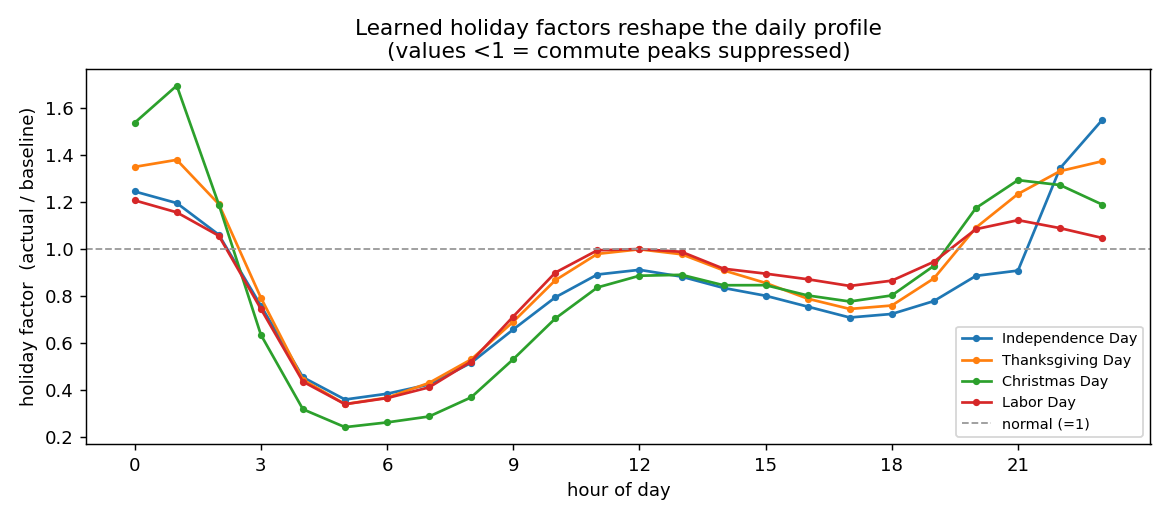
\includegraphics[width=0.92\linewidth]{fig6_holiday_shape.png}
\caption{Learned pooled holiday factors by hour-of-day. Values $<1$ suppress the
commute peaks; the late-evening values $>1$ reflect holiday-eve travel.}
\label{fig:shape}
\end{figure}

\subsection{Results}
Table~\ref{tab:prog} gives the full progression. The holiday model cuts
holiday-window RMSE from $67$ to $48\veh$ ($-29\%$), leaves ordinary hours
exactly unchanged (it only touches special days), and \textbf{stacks} with the
EWMA baseline because the two fixes are orthogonal -- EWMA improves ordinary
hours via recency weighting, the holiday model fixes holidays. Combined:
$R^2=0.9493$, our first clear step past the baseline wall.

\begin{table}[H]
\centering
\caption{Rolling-origin backtest, 2019 (359 origins $\times H{=}168$, holiday
factors from 2017--18). RMSE in \veh.}
\label{tab:prog}
\begin{tabular}{lcccc}
\toprule
Model & $R^2$ (all) & RMSE all & RMSE ordinary & RMSE holiday \\
\midrule
Flat baseline                 & 0.9404 & 40.14 & 37.06 & 66.96 \\
EWMA $\alpha{=}0.8$           & 0.9435 & 39.10 & 35.98 & 65.99 \\
Flat $+$ holiday              & 0.9460 & 38.20 & 37.06 & 49.88 \\
EWMA $+$ holiday (pooled)     & 0.9493 & 37.01 & 35.98 & 47.71 \\
EWMA $+$ holiday (per-sensor) & \textbf{0.9496} & \textbf{36.91} & 35.98 & 46.69 \\
\bottomrule
\end{tabular}
\end{table}

\subsection{Corridor heterogeneity}
A pooled factor assumes every corridor reacts to a holiday identically. It does
not: Figure~\ref{fig:het} shows the distribution of per-sensor holiday
\emph{scale} (a per-sensor multiplier on the pooled factor, shrunk toward 1).
On Thanksgiving, $31\%$ of corridors \emph{gain} traffic (scale up to
$\times1.5$ on recreational routes such as US-101 N), while commute routes drop.
Adding per-sensor scales (shrinkage $\tau=200$) improves $R^2$ only from
$0.9493$ to $0.9496$: with just two holiday instances per sensor the estimates
are noisy and must be shrunk heavily toward the pooled value. This is a
\textbf{``needs more years'' refinement} -- it should pay off once post-2022
data is added.

\begin{figure}[H]
\centering
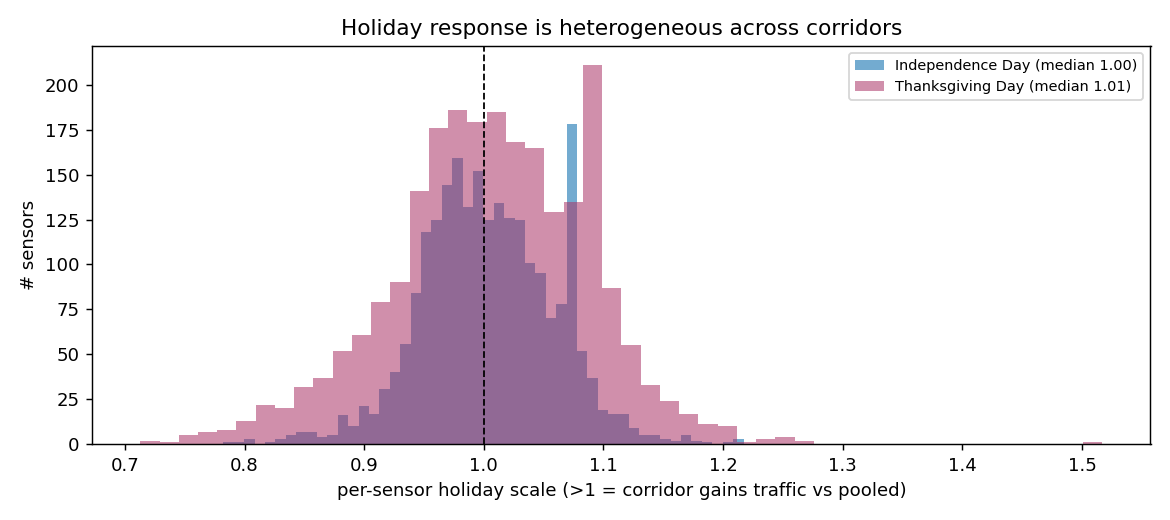
\includegraphics[width=0.92\linewidth]{fig7_holiday_heterogeneity.png}
\caption{Per-sensor holiday scale (multiplier on the pooled factor). The spread,
especially Thanksgiving's gain tail $>1$, is real corridor heterogeneity, but
noisy at two training instances.}
\label{fig:het}
\end{figure}

\section{Does autoregression help? Bounding the residual's own predictability}
\label{sec:next}
Every gain so far comes from the deterministic level (baseline, EWMA, holiday);
none exploits the residual's \emph{own} dynamics, despite its strong short-range
autocorrelation (Note 01: lag-1 $\approx0.81$). Does an autoregressive / ARIMA
correction on the residual add anything under our \textbf{week-aggregate} error
metric? We bound it two ways; both are small.

\subsection{Recent (sub-weekly) lags help only at short horizons}
At origin $t$ forecasting $s=t+h$, a lag-$\ell$ residual $r_{i,s-\ell}$ is
observed iff $\ell\ge h$: a one-day lag is usable only for $h\le24$, a one-hour
lag only for $h=1$. The freshest usable information ages with the horizon (and a
recursive AR(1) is useless, decaying as $0.81^{h}\!\to\!0$). The natural model
is a \emph{direct, per-horizon} regression
$\hat r_{i,t+h}=f_h(\{r_{i,t+h-\ell}:\ell\ge h\})$ added to the baseline.

We measured its ceiling: for each $h$, the residual variance explained by the
best linear predictor on the available lags (train 2017--18, test 2019;
Figure~\ref{fig:hcurve}). It is strong but \emph{collapses} with horizon --
$R^2=0.63$ at $h{=}1$, $0.09$ at $h{=}24$, $0.009$ at $h{=}168$ -- averaging
$0.15$ over the first day but only $0.02$ beyond it. Scaled by the residual's
$6.6\%$ share of total variance and averaged over the week, the best-case lift
in \textbf{aggregate} $R^2$ is just $\mathbf{+0.0027}$
($0.9493\to\sim0.9520$) -- and that is an unreachable ceiling. The signal is
front-loaded into the first day, so a week-aggregate metric dilutes it
roughly $7{:}1$. Worth it only if short horizons (day-ahead, nowcasting) are
scored explicitly.

\begin{figure}[H]\centering
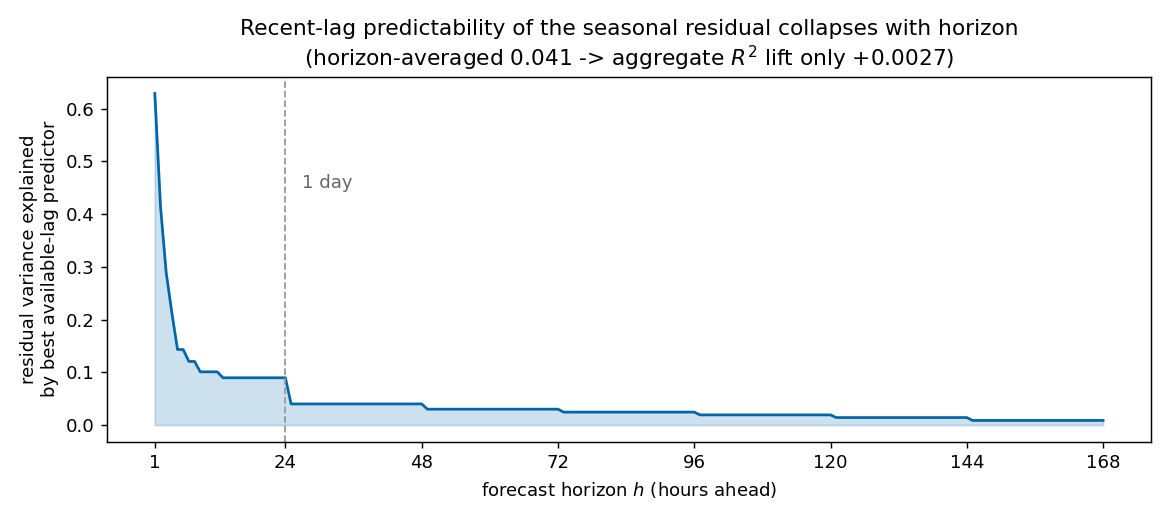
\includegraphics[width=0.9\linewidth]{fig8_horizon_predictability.png}
\caption{Residual variance recoverable from available lags vs.\ forecast
horizon. Huge at $h{=}1$ ($0.63$), gone by a week out -- the value lives in the
first day and is diluted by a week-aggregate metric.}
\label{fig:hcurve}\end{figure}

\subsection{Weekly aggregation: cleaner signal, still small}
A week-\emph{level} forecast would instead help all horizons uniformly, escaping
the dilution. We aggregate the hourly residual to a weekly mean $m_{i,w}$ (within-
week noise cancels), fit an AR on the weekly series, and would re-distribute it
by historical hourly shape. Aggregation does sharpen the signal: the weekly-
aggregate ACF at one week is $\mathbf{+0.295}$ (vs.\ $0.094$ at the hourly
lag-168), with a genuine $+0.36$ load on last week. But only $\mathbf{14.8\%}$
of the residual variance is week-level coherent -- the rest is within-week noise
that cancels and therefore cannot be forecast -- and the weekly series is only
$\sim$10\% predictable out-of-sample. The best-case aggregate lift is
$\mathbf{+0.0010}$, much of it already captured by the EWMA baseline's recency
weighting.

\subsection{Verdict and next directions}
Bounding the autoregressive headroom from both ends -- sub-weekly ($+0.0027$,
diluted) and weekly ($+0.0010$, redundant) -- gives the same answer:
\textbf{small}. The cause is structural: beyond the seasonal baseline and
holidays, the residual is $\sim$90\% within-week idiosyncratic noise (incidents,
weather, one-off events). Traffic is very regular week to week, so its own past
carries little extra; we consider the ARIMA avenue \textbf{closed for the week-
aggregate metric}. The remaining leverage is \textbf{exogenous, all-horizon
signals} that inject new information:
\begin{itemize}
\item \textbf{Weather} (top): precipitation/temperature, forecastable a week
  ahead, depresses flow across a whole week -- the all-horizon shape that made
  holidays pay.
\item Special events, construction and closures (calendar-known); long-run
  growth/trend.
\item Special events, construction and closures (calendar-known); long-run
  growth/trend.
\end{itemize}

\section{Do learned residual features (ridge / XGBoost) help?}
\label{sec:feat}
Before concluding, we test the natural ML escalation: a model (ridge, or XGBoost
for interactions) on the seasonal residual with calendar and sensor-type fixed
effects -- hour-of-week, day-of-week, hour-of-day, week-of-year, and lane count.
For a categorical feature the best predictor is its group mean, so the
out-of-sample variance explained by group means (fit 2017--18, test 2019)
\emph{upper-bounds} what any such model can achieve. The result
(Table~\ref{tab:feat}) is decisive: the sub-daily calendar features explain
$\approx0$ \textbf{by construction} -- the baseline already \emph{is} the
per-sensor hour-of-week mean, so the residual is orthogonal to them. Only
week-of-year carries any signal ($+0.0005$ aggregate), it is largely redundant
with the holiday model, and its sensor-type interaction (XGBoost's supposed edge)
adds nothing; the high-cardinality week-of-year$\times$sensor feature
\emph{overfits} to $-0.045$ out-of-sample. ML cannot manufacture signal that the
construction already removed.

\begin{table}[H]
\centering
\caption{Out-of-sample residual variance explained by each feature's group means
(upper bound for any ridge/XGBoost model on that feature). Test 2019.}
\label{tab:feat}
\begin{tabular}{lcc}
\toprule
Feature on the residual & OOS residual $R^2$ & Aggregate $R^2$ lift \\
\midrule
hour-of-week / day-of-week / hour-of-day & $\le 0$ & $0$ \\
month-of-year (12)            & $+0.001$ & $+0.0001$ \\
week-of-year (52)             & $+0.008$ & $+0.0005$ \\
week-of-year $\times$ lanes   & $+0.009$ & $+0.0005$ \\
week-of-year $\times$ sensor  & $-0.045$ & (overfits) \\
\bottomrule
\end{tabular}
\end{table}

\section{How close are we to the ceiling? Floor and MAPE}
\label{sec:floor}
Two final checks ask whether the problem is, for practical purposes, solved.

\subsection{An irreducible-noise floor}
We estimate the variance no week-ahead model can explain by fitting \emph{oracle}
structure \emph{in-sample} on the 2019 test year itself (perfect parameters, no
estimation error -- an upper bound on achievable skill). Table~\ref{tab:floor}
gives the result. A perfect static weekly-seasonal mean reaches only
$R^2=0.938$, and adding an oracle holiday effect $0.943$ -- yet our
\emph{out-of-sample} EWMA$+$holiday model already scores $0.949$, \textbf{above
the in-sample static oracle}. The reason is informative: the trailing EWMA tracks
\emph{within-year} nonstationarity (sub-annual level drift) that a single annual
mean cannot. Together with \S6--\S7 (no autoregressive or calendar/sensor feature
recovers more than $\sim$$+0.003$), this is strong evidence that the remaining
$\sim$5\% of variance is \textbf{dominated by irreducible idiosyncratic
fluctuation} -- incidents, weather, one-off events -- not learnable structure. We
are near the practical ceiling for \emph{endogenous} information; the one untested
exogenous lever is weather (Note 03 scope), expected to be small for \emph{flow}.

\begin{table}[H]
\centering
\caption{Oracle in-sample fits on 2019 (upper bounds), vs.\ our out-of-sample model.}
\label{tab:floor}
\begin{tabular}{lc}
\toprule
Predictor (oracle = fit on test year) & $R^2$ \\
\midrule
Oracle static weekly-seasonal mean        & 0.9378 \\
\;\; $+$ oracle holiday effect            & 0.9433 \\
Our out-of-sample EWMA $+$ holiday        & \textbf{0.9493} \\
\bottomrule
\end{tabular}
\end{table}

\subsection{The metric: weekly-aggregate MAPE}
The project's headline metric is the weekly-aggregate MAPE (per sensor-week
total). Under it, EWMA$+$holiday scores \textbf{3.55\%} (vs.\ $3.68\%$ flat) --
a strong number. By contrast the \emph{hourly} MAPE looks alarming ($82\%$), but
Figure~\ref{fig:mape} shows this is entirely a small-denominator artifact:
low-flow night hours ($<50\veh$, $13\%$ of points) carry a $583\%$ MAPE, while
peak hours ($>300\veh$, the volume that matters) sit at $6.7\%$. This both
confirms the model is accurate where volume is meaningful and \emph{vindicates
aggregating to the week}, which removes the pathology. (A volume-weighted or
sMAPE metric would do the same at the hourly level.)

\begin{figure}[H]\centering
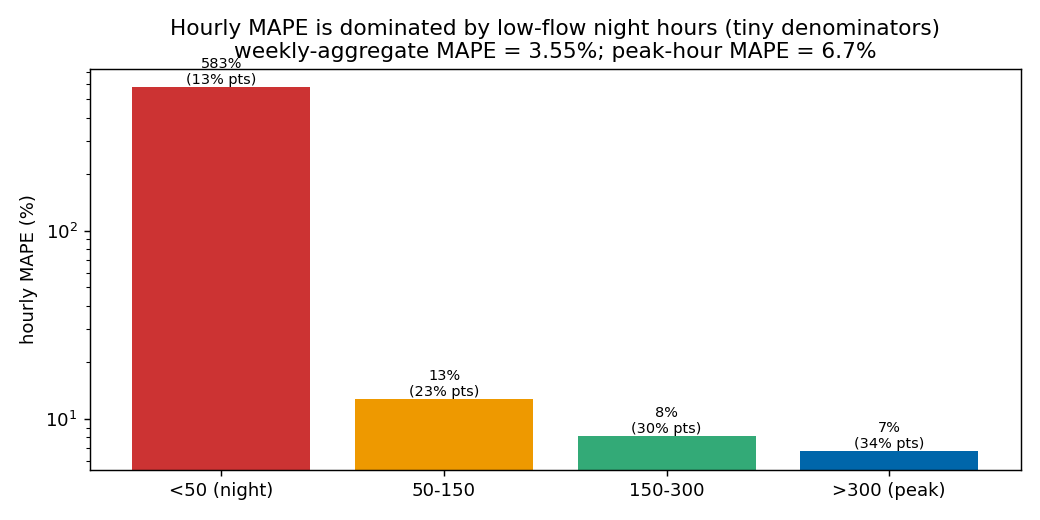
\includegraphics[width=0.82\linewidth]{fig9_mape_regime.png}
\caption{Hourly MAPE by flow regime (log scale). The $82\%$ pooled hourly MAPE is
driven by low-flow night hours with tiny denominators; on peak hours it is
$6.7\%$. Weekly aggregation (denominator = weekly total) avoids this entirely.}
\label{fig:mape}
\end{figure}

\subsection{Verdict}
For Greater Bay Area flow, pre-COVID, the one-week-ahead problem is
\textbf{effectively solved by a simple, interpretable model}: an EWMA seasonal
baseline plus an explicit holiday adjustment, at $R^2=0.949$ and weekly-aggregate
MAPE $3.55\%$, sitting at the practical ceiling for endogenous information. The
open questions are now about \emph{scope} rather than model class: the small
weather lever (Note 03), and generalization beyond this slice -- the COVID-era
2020 regime, post-2022 data, other regions, and \emph{speed} (a genuinely harder
target at $R^2\approx0.76$).

\paragraph{Reproducibility.} All numbers and figures come from the
\texttt{src/} scripts in the project repository (calendar models in
\texttt{holiday\_*} and \texttt{ewma\_baseline}; \S6 headroom in
\texttt{horizon\_ceiling} and \texttt{weekly\_aggregate\_headroom}; \S7 feature
merit in \texttt{feature\_merit}; \S8 floor and MAPE in \texttt{floor\_and\_mape}).

\end{document}
